
\chapter{RADICI DI UN EQUAZIONE}
\section{Esercizio 5}

\textit{\textbf{Descrizione:} Scrivere function Matlab distinte che implementino efficientemente i seguenti metodi per la ricerca degli zeri di una funzione:
\begin{itemize}
\item metodo di bisezione 
\item metodo di Newton
\item metodo delle secanti 
\item metodo delle corde
\end{itemize}
Detta $x_{i}$ l'approssimazione al passo i-esimo, utilizzando come criterio di arresto $\left | \Delta x_{i} \right |\leq tol \cdot (1 + \left | x_{i} \right |)$ essendo $tol$ una opportuna tolleranza specificata in ingresso.}\newpage
\emph{Soluzione: }\\~\\
\textbf{il metodo di bisezione:}
\\~\\
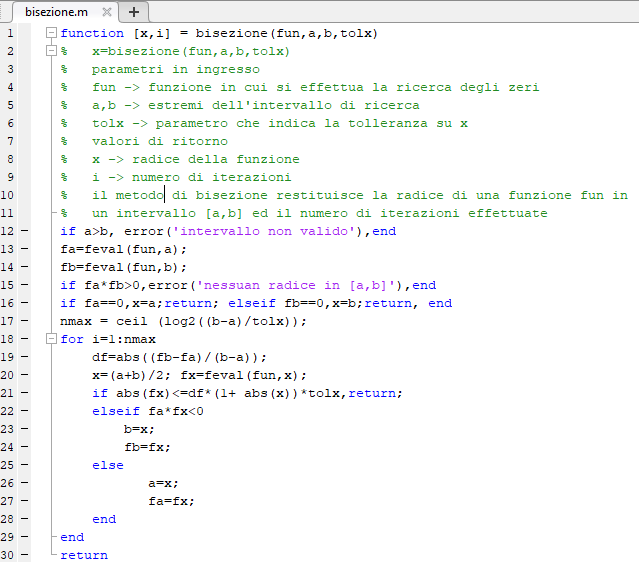
\includegraphics[width=1.3\linewidth]{bisezione} \newpage
\textbf{il metodo di Newton:}
\\~\\
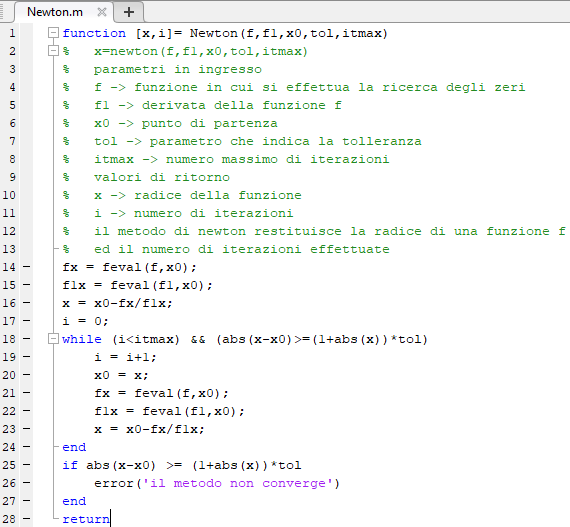
\includegraphics[width=1.3\linewidth]{newton}\newpage
\textbf{il metodo delle secanti:}
\\~\\
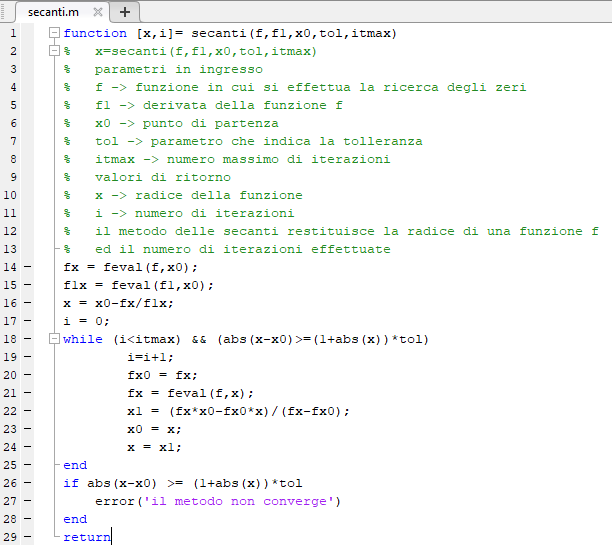
\includegraphics[width=1.3\linewidth]{secanti}\newpage
\textbf{il metodo delle corde:}
\\~\\
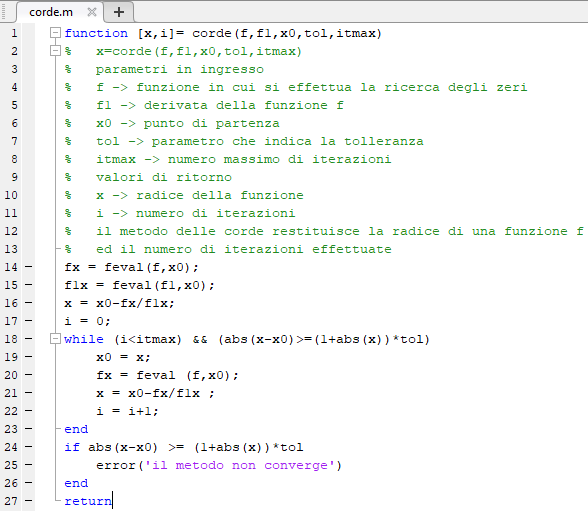
\includegraphics[width=1.3\linewidth]{corde}\newpage

\section{Esercizio 6}

\textit{\textbf{Descrizione:} Utilizzare le function del precedente esercizio per determinare una approssimazione della radice della funzione
$f(x) = x - e^{-x}cos(x/100)$,  per $tol = 10^{-i}, \quad i=1, 2,...,12$, partendo da $x_{0} = -1$. Per il metodo di bisezione,
utilizzare $[-1, 1]$, come intervallo di confidenza iniziale. Tabulare i risultati, in modo da confrontare le iterazioni richieste da ciascun metodo. Commentare il relativo costo computazionale.}\\~\\
\emph{Soluzione: }\\~\\

\makebox[\textwidth][c]{
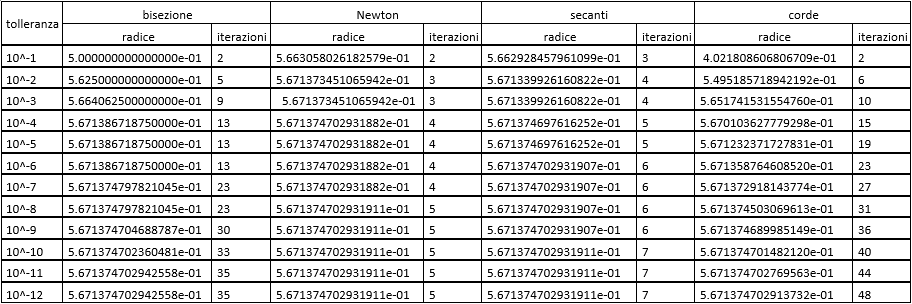
\includegraphics[width=1.3\textwidth]{tabella}
}
\\~\\
Nella tabella sono riportate le radici ricavate con ogni metodo e il relativo numero di iterazioni necessarie per ottenere tale risultato per ogni $tol = 10^{-i}, \quad i=1, 2,...,12$.\newline
Il metodo di bisezione e il metodo delle corde hanno una valutazione di funzione e convergenza lineare mentre il metodo di Newton ha due valutazioni di funzioni, una per la funzione e una per la sua derivata, e convergenza quadratica quindi col metodo di Newton si ha una maggiore velocit\'a nella ricerca della radice ma si ha anche un costo computazionale maggiore. Il metodo delle secanti ha una valutazione di funzione, quindi un costo computazionale minore del metodo di Newton,  e una convergenza $\approx$ 1.618, quindi ha una velocit\'a maggiore dei metodi di bisezione e delle secanti.


\section{Esercizio 7}

\textit{\textbf{Descrizione:} Calcolare la molteplicit\'a della radice nulla della funzione $f(x) = x^{2} \cdot sin(x^{2})$. Confrontare, quindi, i metodi di Newton, Newton modificato, e di Aitken, per approssimarla per gli stessi valori di tol del precedente esercizio (ed utilizzando il medesimo criterio di arresto), partendo da $x_{0}=1$. Tabulare e commentare i risultati ottenuti.}\\~\\
\emph{Soluzione:}\\~\\
La molteplicit\'a $m$ della radice nulla della funzione $f(x) = x^{2} \cdot sin(x^{2})$  \'e $m=4$
\\~\\
\textbf{il metodo di Newton modificato:}
\\~\\
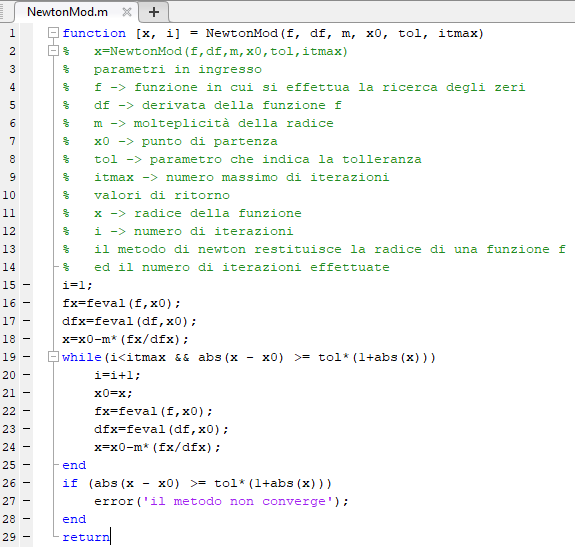
\includegraphics[width=1.3\linewidth]{NewtonMod}\newpage
\textbf{il metodo di aitken:}
\\~\\
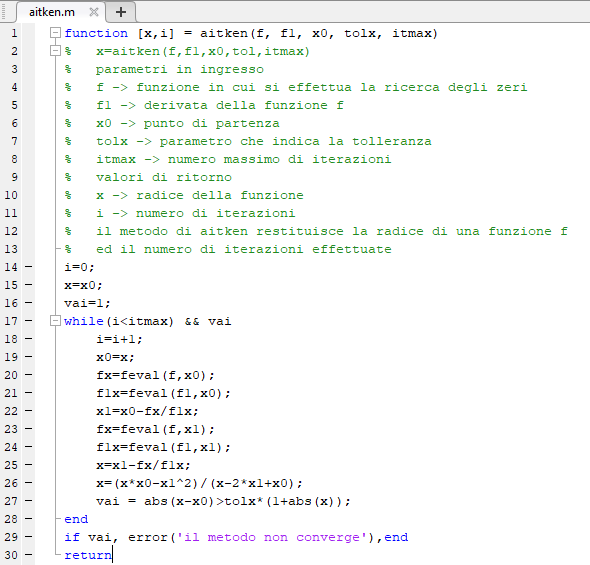
\includegraphics[width=1.3\linewidth]{aitken}\newpage
\makebox[\textwidth][c]{
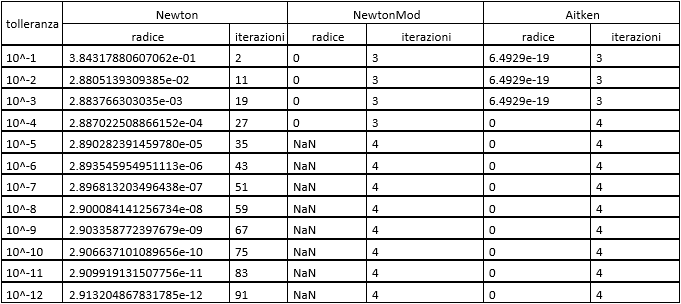
\includegraphics[width=1.3\textwidth]{tabella2}
}